% Options for packages loaded elsewhere
\PassOptionsToPackage{unicode}{hyperref}
\PassOptionsToPackage{hyphens}{url}
%
\documentclass[
  ignorenonframetext,
]{beamer}
\title{GLOBE Leadership and Societal Perspectives}
\subtitle{Ethan Allavarpu \(\cdot\) Raymond Bai \(\cdot\) Jaclyn Chiu
\newline Ariel Chow \(\cdot\) Carlie Lin \(\cdot\) Dara Tan}
\author{\textbf{Explore the GLOBE}}
\date{STATS 140XP \(\cdot\) Fall 2021}

\usepackage{pgfpages}
\setbeamertemplate{caption}[numbered]
\setbeamertemplate{caption label separator}{: }
\setbeamercolor{caption name}{fg=normal text.fg}
\beamertemplatenavigationsymbolsempty
% Prevent slide breaks in the middle of a paragraph
\widowpenalties 1 10000
\raggedbottom
\setbeamertemplate{part page}{
  \centering
  \begin{beamercolorbox}[sep=16pt,center]{part title}
    \usebeamerfont{part title}\insertpart\par
  \end{beamercolorbox}
}
\setbeamertemplate{section page}{
  \centering
  \begin{beamercolorbox}[sep=12pt,center]{part title}
    \usebeamerfont{section title}\insertsection\par
  \end{beamercolorbox}
}
\setbeamertemplate{subsection page}{
  \centering
  \begin{beamercolorbox}[sep=8pt,center]{part title}
    \usebeamerfont{subsection title}\insertsubsection\par
  \end{beamercolorbox}
}
\AtBeginPart{
  \frame{\partpage}
}
\AtBeginSection{
  \ifbibliography
  \else
    \frame{\sectionpage}
  \fi
}
\AtBeginSubsection{
  \frame{\subsectionpage}
}
\usepackage{amsmath,amssymb}
\usepackage{lmodern}
\usepackage{iftex}
\ifPDFTeX
  \usepackage[T1]{fontenc}
  \usepackage[utf8]{inputenc}
  \usepackage{textcomp} % provide euro and other symbols
\else % if luatex or xetex
  \usepackage{unicode-math}
  \defaultfontfeatures{Scale=MatchLowercase}
  \defaultfontfeatures[\rmfamily]{Ligatures=TeX,Scale=1}
\fi
\usetheme[]{Hannover}
\usecolortheme{spruce}
% Use upquote if available, for straight quotes in verbatim environments
\IfFileExists{upquote.sty}{\usepackage{upquote}}{}
\IfFileExists{microtype.sty}{% use microtype if available
  \usepackage[]{microtype}
  \UseMicrotypeSet[protrusion]{basicmath} % disable protrusion for tt fonts
}{}
\makeatletter
\@ifundefined{KOMAClassName}{% if non-KOMA class
  \IfFileExists{parskip.sty}{%
    \usepackage{parskip}
  }{% else
    \setlength{\parindent}{0pt}
    \setlength{\parskip}{6pt plus 2pt minus 1pt}}
}{% if KOMA class
  \KOMAoptions{parskip=half}}
\makeatother
\usepackage{xcolor}
\IfFileExists{xurl.sty}{\usepackage{xurl}}{} % add URL line breaks if available
\IfFileExists{bookmark.sty}{\usepackage{bookmark}}{\usepackage{hyperref}}
\hypersetup{
  pdftitle={GLOBE Leadership and Societal Perspectives},
  hidelinks,
  pdfcreator={LaTeX via pandoc}}
\urlstyle{same} % disable monospaced font for URLs
\newif\ifbibliography
\usepackage{graphicx}
\makeatletter
\def\maxwidth{\ifdim\Gin@nat@width>\linewidth\linewidth\else\Gin@nat@width\fi}
\def\maxheight{\ifdim\Gin@nat@height>\textheight\textheight\else\Gin@nat@height\fi}
\makeatother
% Scale images if necessary, so that they will not overflow the page
% margins by default, and it is still possible to overwrite the defaults
% using explicit options in \includegraphics[width, height, ...]{}
\setkeys{Gin}{width=\maxwidth,height=\maxheight,keepaspectratio}
% Set default figure placement to htbp
\makeatletter
\def\fps@figure{htbp}
\makeatother
\setlength{\emergencystretch}{3em} % prevent overfull lines
\providecommand{\tightlist}{%
  \setlength{\itemsep}{0pt}\setlength{\parskip}{0pt}}
\setcounter{secnumdepth}{-\maxdimen} % remove section numbering
\usepackage{booktabs}
\usepackage{longtable}
\usepackage{array}
\usepackage{multirow}
\usepackage{wrapfig}
\usepackage{float}
\usepackage{colortbl}
\usepackage{pdflscape}
\usepackage{tabu}
\usepackage{threeparttable}
\usepackage{threeparttablex}
\usepackage[normalem]{ulem}
\usepackage{makecell}
\usepackage{xcolor}
\ifLuaTeX
  \usepackage{selnolig}  % disable illegal ligatures
\fi

\begin{document}
\frame{\titlepage}

\hypertarget{introducing-the-data}{%
\section{Introducing the Data}\label{introducing-the-data}}

\begin{frame}{The Data}
\protect\hypertarget{the-data}{}
\begin{itemize}
\tightlist
\item
  GLOBE (Global Leadership \& Organizational Behavior Effectiveness)

  \begin{itemize}
  \tightlist
  \item
    Goal: Identify the relationships between various leadership and
    societal characteristics
  \item
    Over 17,000 middle managers, 62 cultures
  \item
    Leadership survey from 1 (negative) to 7 (positive)
  \item
    Societal survey not necessarily coded the same as leadership

    \begin{itemize}
    \tightlist
    \item
      Did not end up affecting our analysis
    \item
      Only cared about relationships between variables
    \item
      Societal coded the same way for a given characteristic
    \end{itemize}
  \end{itemize}
\item
  Outside source: ISO Codes from Wikipedia

  \begin{itemize}
  \tightlist
  \item
    Uniform identifiers for countries for visualization purposes
  \end{itemize}
\end{itemize}
\end{frame}

\begin{frame}{Exploratory Data Analysis}
\protect\hypertarget{exploratory-data-analysis}{}
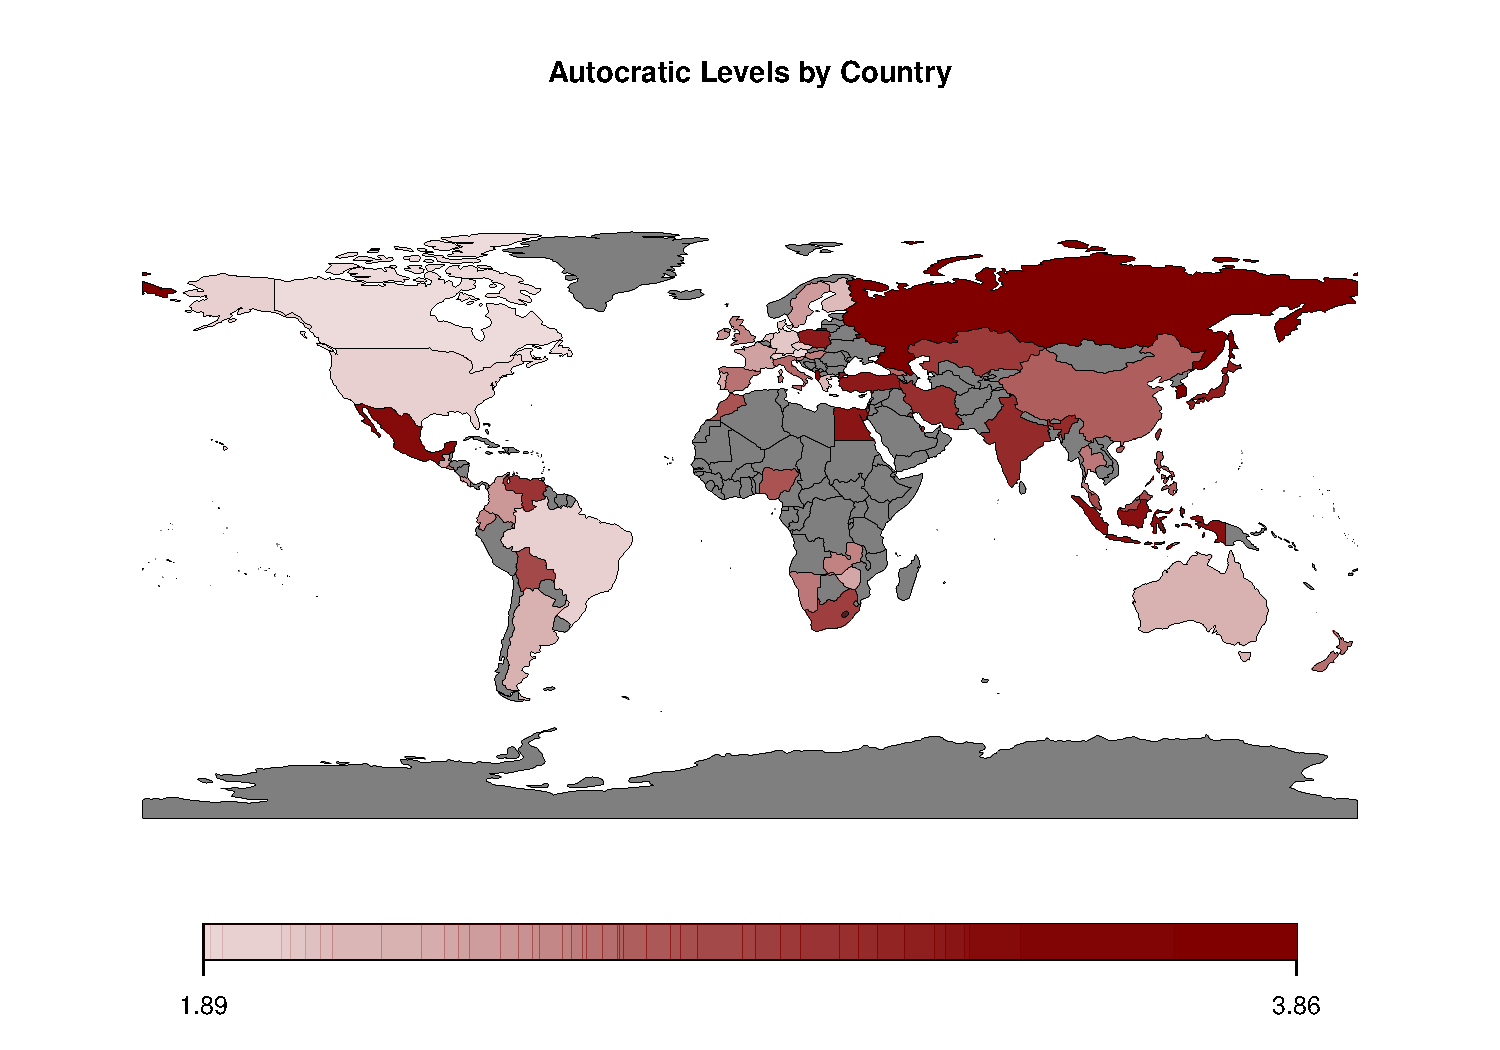
\includegraphics{final_slides_files/figure-beamer/eda_leader-1.pdf}
\end{frame}

\begin{frame}{Exploratory Data Analysis}
\protect\hypertarget{exploratory-data-analysis-1}{}
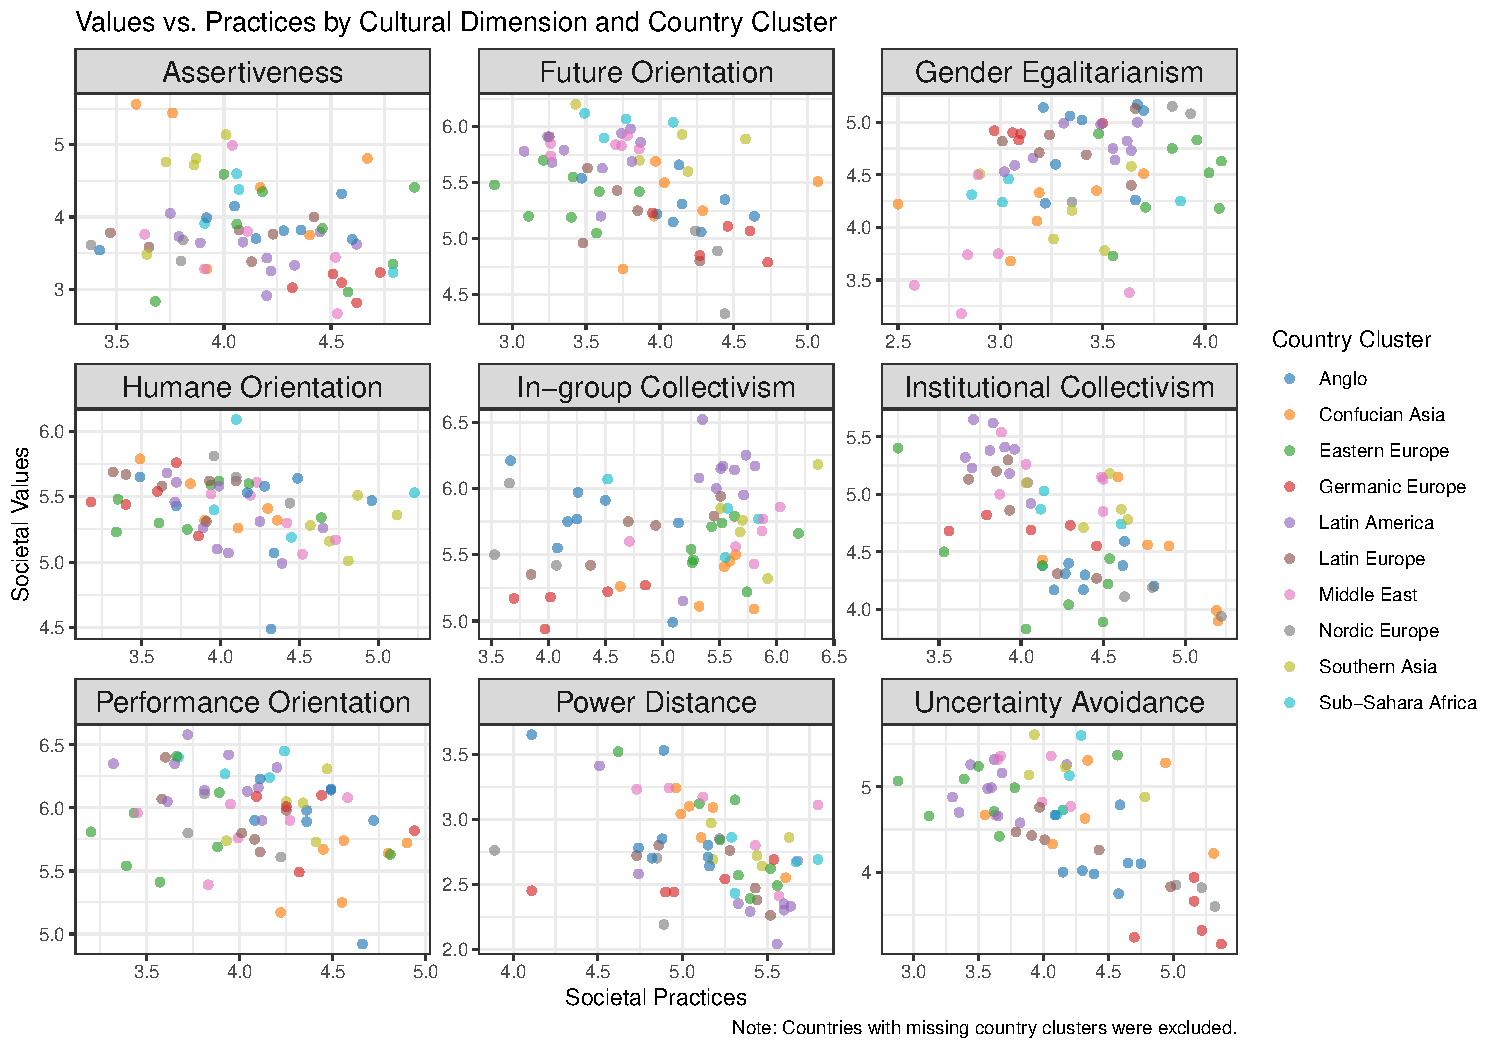
\includegraphics{final_slides_files/figure-beamer/eda_social-1.pdf}
\end{frame}

\begin{frame}{Problem Statements}
\protect\hypertarget{problem-statements}{}
\begin{enumerate}
\tightlist
\item
  Which characteristics or traits do countries tend to group together
  when determining ``good'' leadership values?

  \begin{itemize}
  \tightlist
  \item
    Which countries have similar perceptions of these leadership values?
  \end{itemize}
\item
  Do societal practices and societal values align?

  \begin{itemize}
  \tightlist
  \item
    If they do not, which practices and values deviate most
    significantly?
  \end{itemize}
\end{enumerate}
\end{frame}

\hypertarget{analysis}{%
\section{Analysis}\label{analysis}}

\begin{frame}{Leadership Clusters: Methodology}
\protect\hypertarget{leadership-clusters-methodology}{}
\begin{enumerate}
\item
  Remove second-order factor analysis variables (difficult for
  interpretation)
\item
  Perform PCA on the remaining numeric variables
\item
  Perform \(k\)-means clustering on the first four principal components
  for both characteristics and countries

  \begin{itemize}
  \tightlist
  \item
    Choose first four PCs because they explain around 80\% of the
    variation
  \end{itemize}
\end{enumerate}
\end{frame}

\begin{frame}{Leadership Clusters: Methodology}
\protect\hypertarget{leadership-clusters-methodology-1}{}
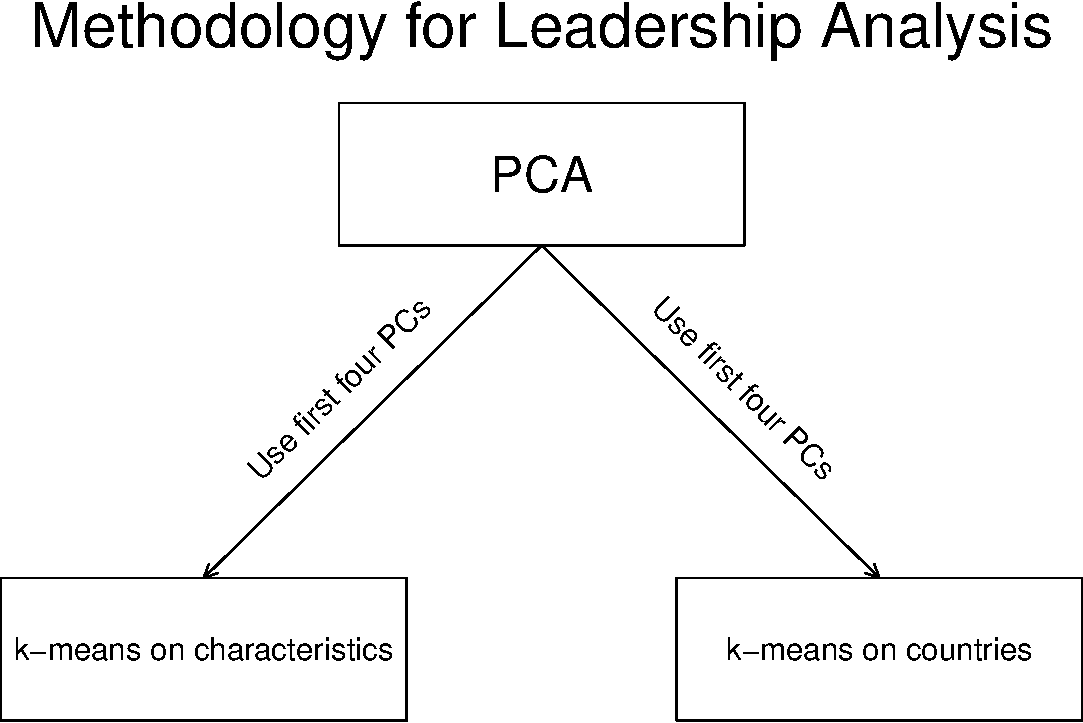
\includegraphics{final_slides_files/figure-beamer/leader_methods-1.pdf}
\end{frame}

\begin{frame}{Leadership Clusters: Characteristics}
\protect\hypertarget{leadership-clusters-characteristics}{}
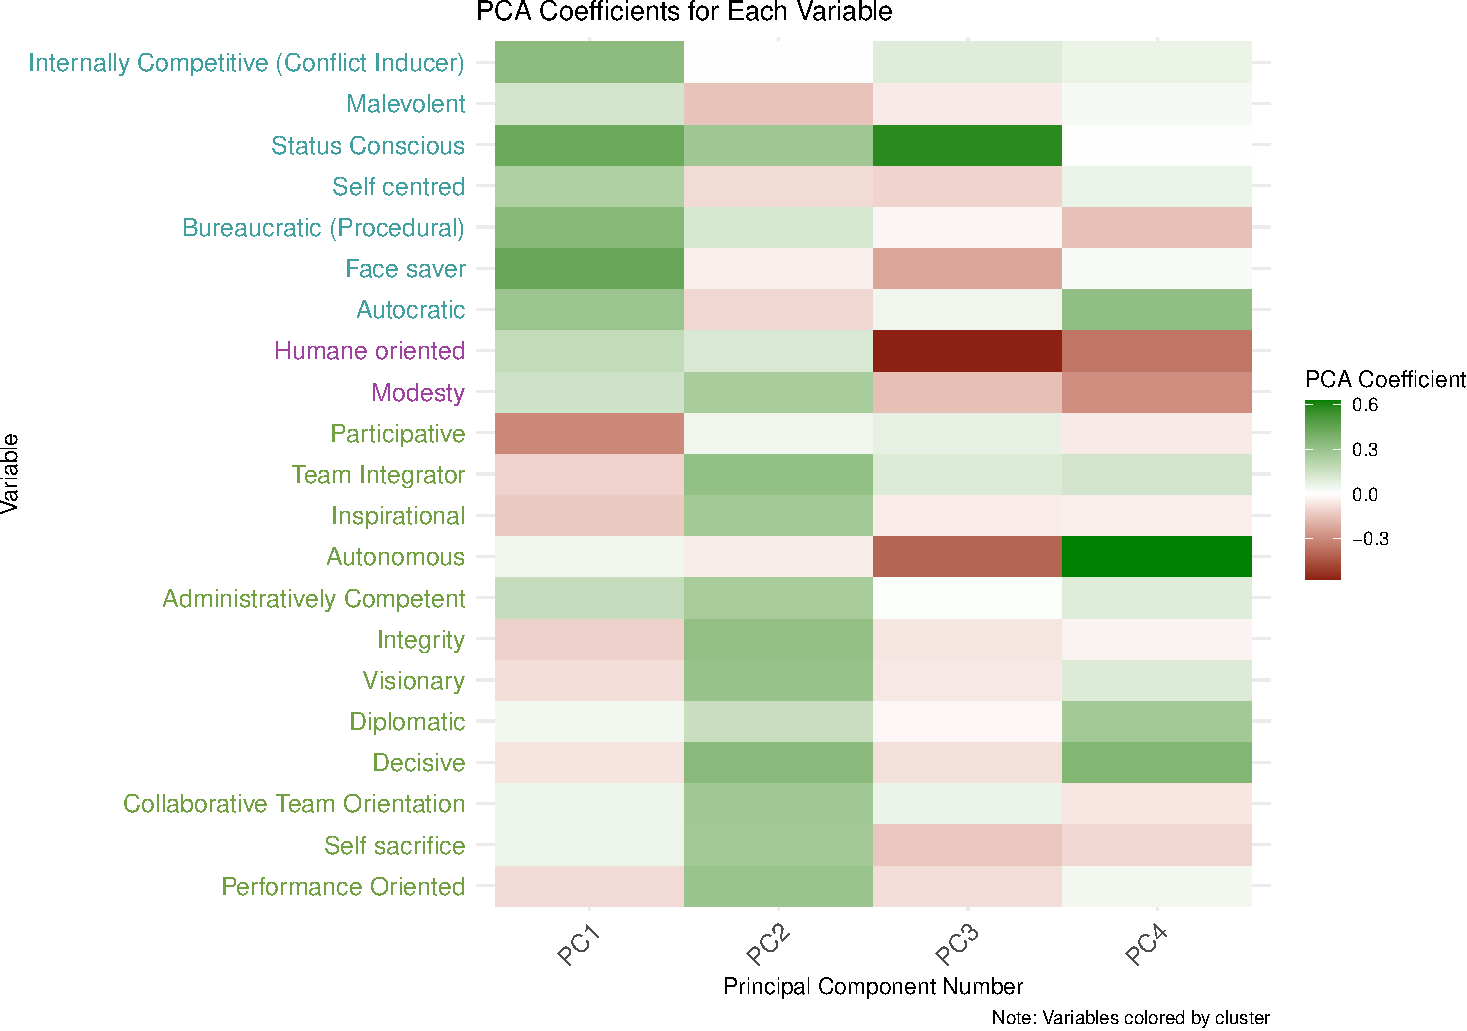
\includegraphics{final_slides_files/figure-beamer/pca_heatmap-1.pdf}
\end{frame}

\begin{frame}{Leadership Clusters: Characteristics}
\protect\hypertarget{leadership-clusters-characteristics-1}{}
\definecolor{clust3}{HTML}{408000}
\definecolor{clust2}{HTML}{800080}
\definecolor{clust1}{HTML}{008080}

\begin{enumerate}
\item
  \textcolor{clust1}{Internally competitive, malevolent, status conscious, self-centred, bureaucratic, face saver, autocratic}

  \begin{itemize}
  \tightlist
  \item
    Negative characteristics
  \end{itemize}
\item
  \textcolor{clust2}{Humane-oriented, modesty}

  \begin{itemize}
  \tightlist
  \item
    Distinctly different group of two
  \end{itemize}
\item
  \textcolor{clust3}{Participative, team integrator, inspirational, autonomous, administratively competent, integrity, visionary, diplomatic, decisive, collaborative team orientation, self-sacrifice, performance-oriented}

  \begin{itemize}
  \tightlist
  \item
    Positive characteristics
  \end{itemize}
\end{enumerate}
\end{frame}

\begin{frame}{Leadership Clusters: Countries}
\protect\hypertarget{leadership-clusters-countries}{}
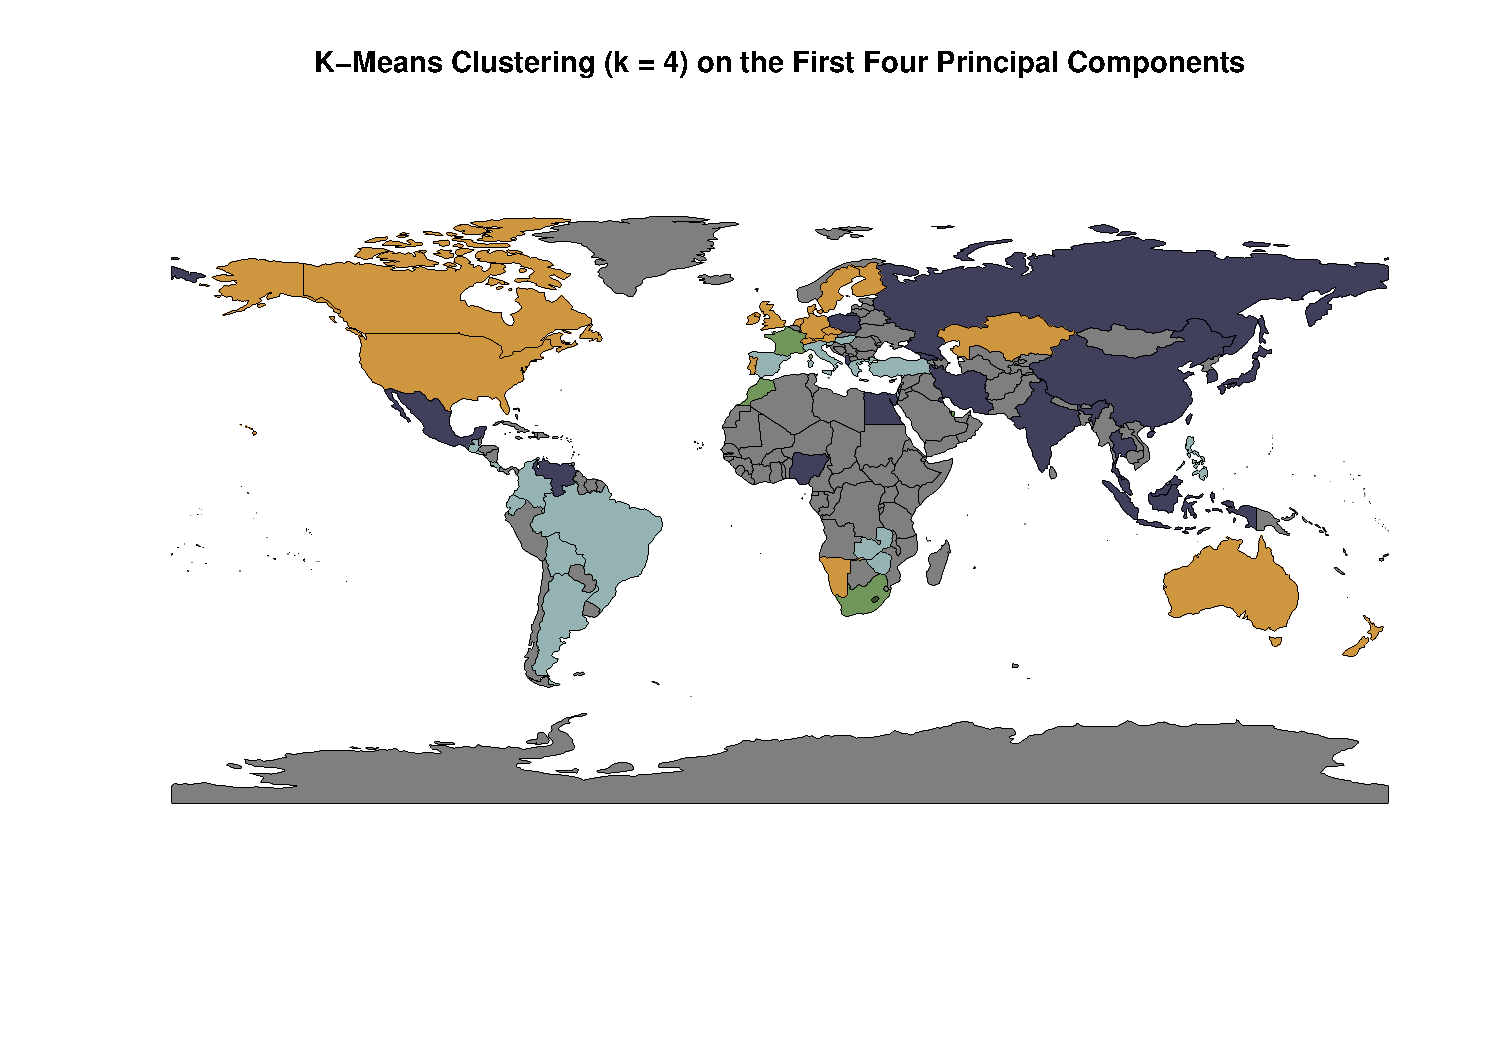
\includegraphics{final_slides_files/figure-beamer/kmeans-1.pdf}

\emph{Note: East, West Germany in the same cluster. South Africa colored
by Black sample (rather than the White sample)}
\end{frame}

\begin{frame}{Leadership Clusters: Countries}
\protect\hypertarget{leadership-clusters-countries-1}{}
\definecolor{clust4}{HTML}{739999}
\definecolor{clust5}{HTML}{000026}
\definecolor{clust6}{HTML}{407326}
\definecolor{clust7}{HTML}{BF7300}

\begin{itemize}
\tightlist
\item
  \textcolor{clust4}{Light Blue}: Latin America, Mediterranean
\item
  \textcolor{clust5}{Dark Blue}: Asia
\item
  \textcolor{clust6}{Green}: No specific regionality
\item
  \textcolor{clust7}{Gold}: Western and Northern Europe, Anglo
\end{itemize}
\end{frame}

\begin{frame}{Leadership Clusters}
\protect\hypertarget{leadership-clusters}{}
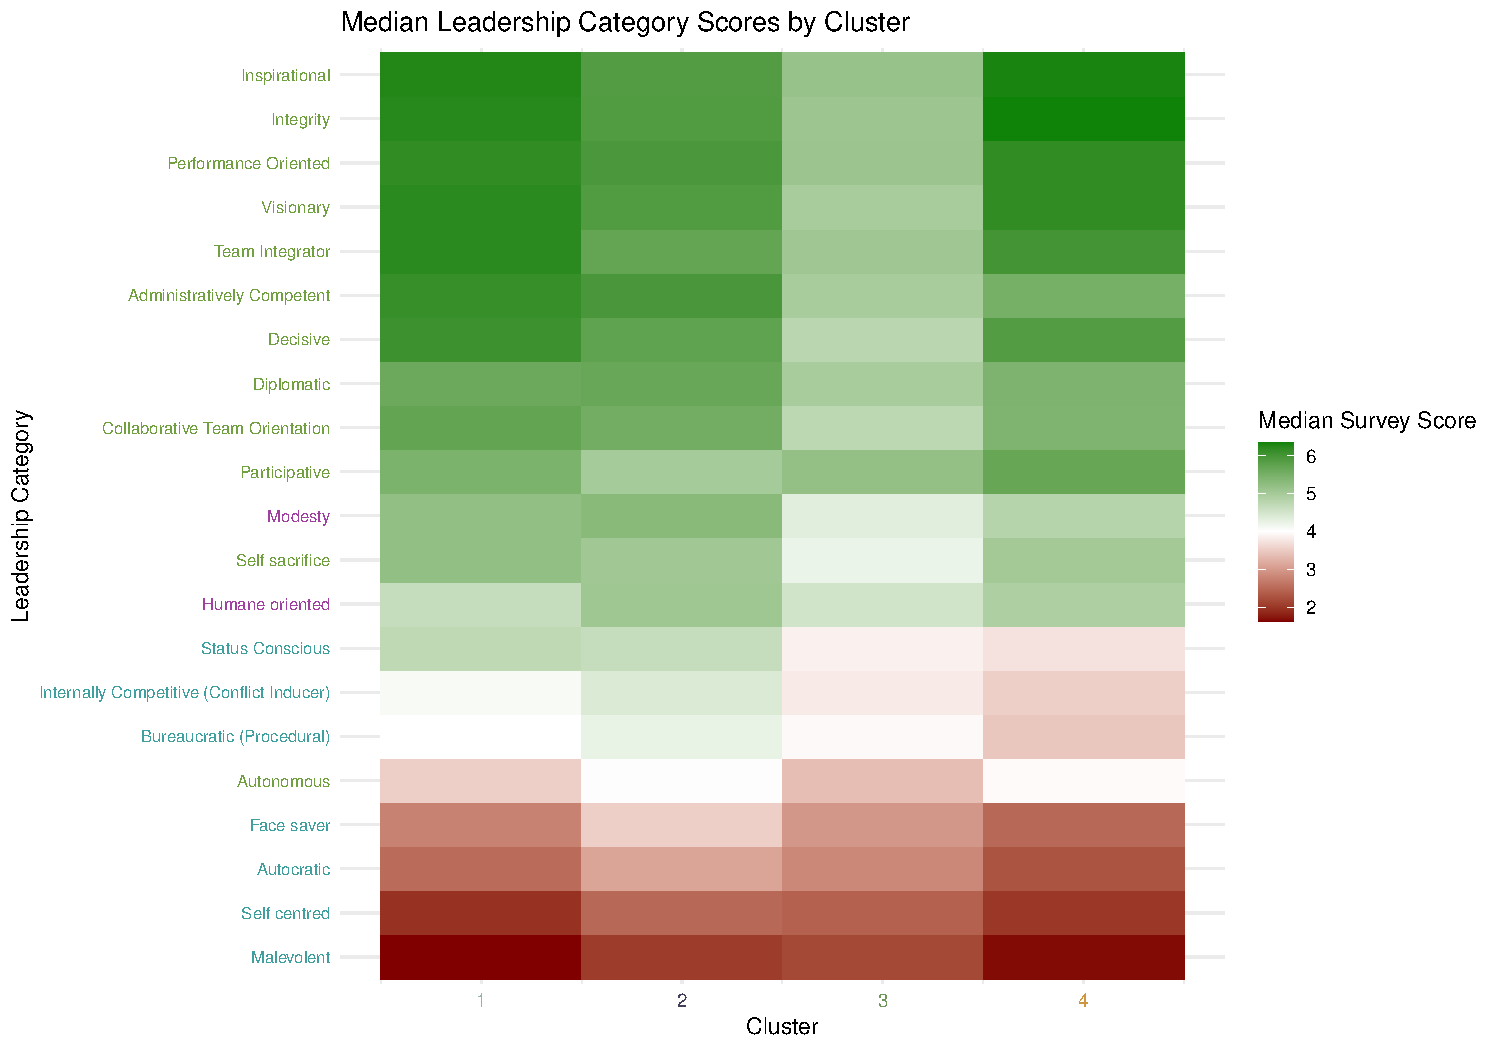
\includegraphics{final_slides_files/figure-beamer/cluster_values-1.pdf}
\end{frame}

\begin{frame}{Societal Values vs.~Practices: Methodology}
\protect\hypertarget{societal-values-vs.-practices-methodology}{}
For each cultural dimension:

\begin{itemize}
\item
  Simple linear regression model: \(y = \beta_0 + \beta_1 x\)
\item
  \(t\)-test: \(H_0: \beta_1 = 0\) versus \(H_1: \beta_1 \ne 0\)
\item
  Bonferroni Correction

  \begin{itemize}
  \tightlist
  \item
    Change significance threshold from \(\alpha = 0.05\) to
    \(\alpha = \frac{0.05}{9} \approx 0.0056\)
  \end{itemize}
\end{itemize}
\end{frame}

\begin{frame}{Societal Values vs.~Practices: Findings}
\protect\hypertarget{societal-values-vs.-practices-findings}{}
\begin{table}[!h]

\caption{\label{tab:SPV SLR Table}Results of Simple Linear Regression by Cultural Dimension}
\centering
\begin{tabular}[t]{lrr}
\toprule
Cultural Dimension & Coefficient Value & p-value\\
\midrule
\cellcolor[HTML]{E5F5E0}{Uncertainty Avoidance} & \cellcolor[HTML]{E5F5E0}{-0.6199} & \cellcolor[HTML]{E5F5E0}{0.0000}\\
\cellcolor[HTML]{E5F5E0}{Institutional Collectivism} & \cellcolor[HTML]{E5F5E0}{-0.5251} & \cellcolor[HTML]{E5F5E0}{0.0000}\\
\cellcolor[HTML]{E5F5E0}{Power Distance} & \cellcolor[HTML]{E5F5E0}{-0.4991} & \cellcolor[HTML]{E5F5E0}{0.0006}\\
\cellcolor[HTML]{E5F5E0}{Future Orientation} & \cellcolor[HTML]{E5F5E0}{-0.4725} & \cellcolor[HTML]{E5F5E0}{0.0009}\\
Humane Orientation & -0.5944 & 0.0116\\
\addlinespace
\cellcolor[HTML]{F0F0F0}{Gender Egalitarianism} & \cellcolor[HTML]{F0F0F0}{0.2437} & \cellcolor[HTML]{F0F0F0}{0.0124}\\
Performance Orientation & -0.3459 & 0.0268\\
\cellcolor[HTML]{F0F0F0}{Assertiveness} & \cellcolor[HTML]{F0F0F0}{-0.1507} & \cellcolor[HTML]{F0F0F0}{0.0414}\\
In-group Collectivism & 0.4393 & 0.0991\\
\bottomrule
\end{tabular}
\end{table}
\end{frame}

\hypertarget{conclusions}{%
\section{Conclusions}\label{conclusions}}

\begin{frame}{Leadership Clusters}
\protect\hypertarget{leadership-clusters-1}{}
\definecolor{clust2}{HTML}{800080}
\definecolor{clust6}{HTML}{407326}

\begin{itemize}
\tightlist
\item
  Characteristics clustered largely on negative or positive connotations

  \begin{itemize}
  \tightlist
  \item
    Exceptions: \textcolor{clust2}{Humane oriented, modesty}
  \end{itemize}
\item
  Countries clustered heavily on geographic region

  \begin{itemize}
  \tightlist
  \item
    Exceptions: \textcolor{clust6}{Green cluster}
  \end{itemize}
\end{itemize}
\end{frame}

\begin{frame}{Societal Values vs.~Practices}
\protect\hypertarget{societal-values-vs.-practices}{}
\begin{itemize}
\tightlist
\item
  Practices do not align

  \begin{itemize}
  \tightlist
  \item
    Correlations often negative
  \end{itemize}
\item
  Consider how this might affect policy implementation
\end{itemize}
\end{frame}

\begin{frame}{Further Research}
\protect\hypertarget{further-research}{}
\begin{itemize}
\tightlist
\item
  Investigate how other indices (e.g., freedom index, happiness index,
  government approval ratings) explain groupings for leadership values
\item
  Potential causes behind inverse relationship between societal values
  and practices

  \begin{itemize}
  \tightlist
  \item
    Are people valuing certain things \emph{because} they aren't present
    in the society?
  \end{itemize}
\item
  Expand the survey to more countries to see if regional trends/clusters
  remain
\end{itemize}
\end{frame}

\begin{frame}{Limitations}
\protect\hypertarget{limitations}{}
\begin{itemize}
\tightlist
\item
  Only 62 cultures observed
\item
  Some countries split

  \begin{itemize}
  \tightlist
  \item
    Germany: East vs.~West (possibly related to Berlin Wall)
  \item
    South Africa: White vs.~Black (possibly related to Apartheid)
  \end{itemize}
\item
  Data appears to be from 15+ years ago

  \begin{itemize}
  \tightlist
  \item
    Potentially outdated information
  \item
    May consider a resurvey
  \end{itemize}
\item
  Unsure of how second-order factor analysis performed
\item
  No ``official'' codebook--just found the survey questions
\end{itemize}
\end{frame}

\end{document}
